\documentclass[tikz,border=2pt]{standalone}
\usepackage{amsmath,amssymb}
\usepackage{tikz}
\usetikzlibrary{arrows.meta}

\begin{document}
% An augmenting path in the residual network of a partial flow (value 5): A-C-E-F has
% residual capacities 2, 4, 3, so its bottleneck is 2 and the flow can be raised by 2.
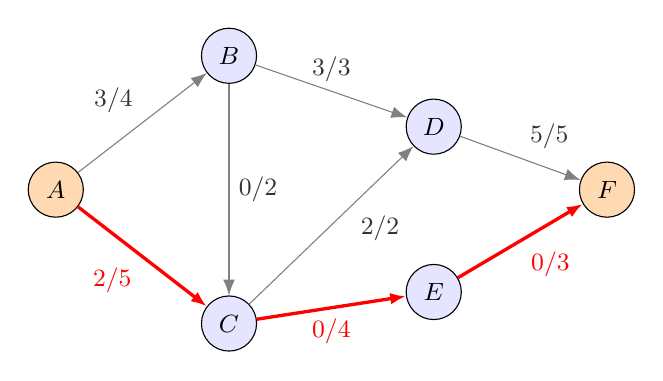
\begin{tikzpicture}[every node/.style={font=\small}, >={Latex[length=2mm]}, v/.style={draw, circle, fill=blue!10, minimum size=7mm, inner sep=0pt}]
	\node[v, fill=orange!30] (A) at (0,0) {$A$};
	\node[v] (B) at (2.2,1.7) {$B$};
	\node[v] (C) at (2.2,-1.7) {$C$};
	\node[v] (D) at (4.8,0.8) {$D$};
	\node[v] (E) at (4.8,-1.3) {$E$};
	\node[v, fill=orange!30] (F) at (7.0,0) {$F$};
	\draw[->, gray] (A) -- (B) node[midway, above left, text=gray!40!black] {$3/4$};
	\draw[->, gray] (B) -- (D) node[midway, above, text=gray!40!black] {$3/3$};
	\draw[->, gray] (C) -- (D) node[pos=0.62, below right, text=gray!40!black] {$2/2$};
	\draw[->, gray] (D) -- (F) node[midway, above right, text=gray!40!black] {$5/5$};
	\draw[->, gray] (B) -- (C) node[midway, right, text=gray!40!black] {$0/2$};
	\draw[->, very thick, red] (A) -- (C) node[midway, below left] {$2/5$};
	\draw[->, very thick, red] (C) -- (E) node[midway, below] {$0/4$};
	\draw[->, very thick, red] (E) -- (F) node[midway, below right] {$0/3$};
	\end{tikzpicture}
\end{document}
